\section{Durchführung und Aufbau}
\label{sec:Durchführung}

\subsection{Versuchsaufbau}
\label{sec:Versuchsaufbau}
Der Aufbau ist in \autoref{fig:aufbau} abgebildet.
\begin{figure}
  \centering
  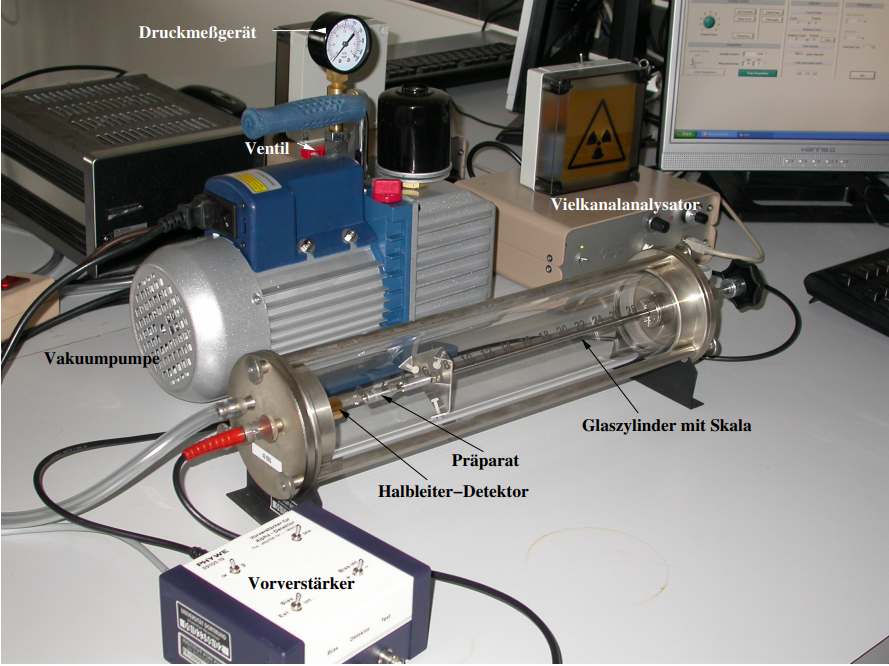
\includegraphics[width=0.8\textwidth]{img/aufbau.png}
  \caption{Versuchsaufbau \cite{anleitung}.}
  \label{fig:aufbau}
\end{figure}

In einer evakuierten Glasröhre befindet sich eine $\ce{^{241}Am}$-Quelle, die $\alpha$-Strahlung emittiert und ein Halbleiter-Sperrschichtzähler, der die Strahlung detektiert.
Der Zerfall der Quelle ist:
\begin{equation*}
  \ce{^{241}_{95}Am -> ^{237}_{93}Np + ^{4}_{2}He^2+}.
\end{equation*}
Der Sperrschichtzähler ist über einen Verstärker mit einem Multichannelanalyzer verbunden. Dieser ist mit einem Computer verbunden, auf dem die Messwerte gespeichert werden.
Der Abstand zwischen Quelle und Zähler kann variiert werden. 

\subsection{Durchführung}
\label{sec:Durchführung}
Bevor die Messung beginnt, muss die Diskriminatorschwelle des Verstärkers so eingestellt werden, dass gerade so eben die $\alpha$-Strahlung detektiert wird.
Zunächst muss der Glaszyliner evakuiert werden. Wenn ein Druck von $p \approx \SI{0}{}$ erreicht ist, kann die Messung beginnen. Der Druck sollte während der Messung konstant bleiben.\\
Die Zählrate sollte aufgrund des geringen Drucks zunnehmen. Es wird die Zählrate der $\alpha$-Strahlung in Abhängigkeit des Drucks gemessen. Dazu wird der Druck in $\SI{50}{\milli\bar}$-Schritten erhöht.
Der Druck wird dabei über ein Ventil geregelt. Die Messzeit beträgt $\SI{120}{\second}$ pro Druck.\\
Bei jedem Druck wird die Position des Energiemaximus und die Gesamtzählrate aufgenommen. Zu Beginn sollte der die Energie des Energiemaximums bei $\SI{4}{\mega\electronvolt}$ liegen.\\
\\
Zusätzlich soll die Statistik des radioaktiven Zerfalls untersucht werden. Dazu wird die Zählrate in Abhängigkeit der Zeit gemessen. Die Messzeit beträgt $\SI{10}{\second}$ pro Messung. Es werden 100 Messungen durchgeführt.\\

